\documentclass[border=4pt]{standalone}
\usepackage[T1]{fontenc}
\usepackage{helvet}
\renewcommand{\familydefault}{\sfdefault}
\usepackage{graphicx}
\usepackage{caption}
\usepackage{amsmath}
\captionsetup{font={sf,footnotesize},labelfont={sf,bf,footnotesize},justification=justified,singlelinecheck=false}
\begin{document}
\setcounter{figure}{3}
\begin{minipage}{7.20in}
\centering
\begin{figure}[htbp]
    \centering
    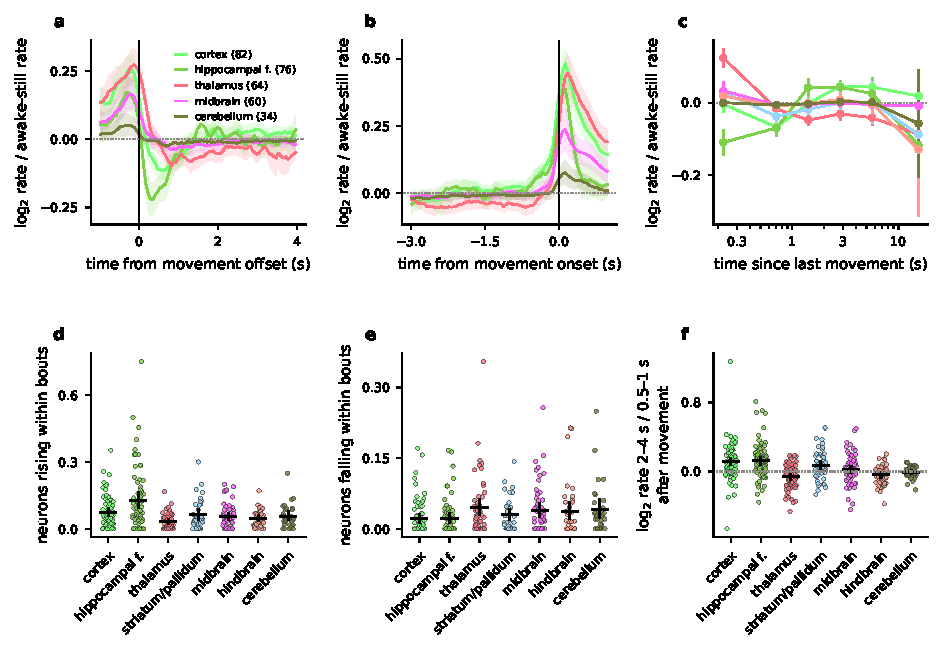
\includegraphics[width=\linewidth]{fig4_dynamics_panels.pdf}
    \caption{Stillness is graded: firing dips after movement ends, then thalamus keeps falling while cortex and hippocampus recover. \textbf{a} Population rate around the end of a movement that starts an awake-still bout of $\geq$4\,s, relative to the awake-still rate; mean over mice (number in legend) and bootstrap 95\% CI, 250\,ms smoothing. \textbf{b} The same around movement onset after $\geq$3\,s of awake stillness. \textbf{c} Rate in awake-still bins by time since the last movement (all bouts), mean over mice $\pm$ 1.96 s.e.m.; colours as in a, plus striatum/pallidum and hindbrain. \textbf{d} Fraction of neurons whose rate rises from the first 0.5\,s to 2--4\,s within $\geq$4\,s bouts (Wilcoxon over bouts, $p<0.01$); dots are mice. \textbf{e} Fraction of neurons whose rate falls. \textbf{f} Rate 2--4\,s vs 0.5--1\,s after the last movement, per mouse.}
    \label{fig:dynamics}
\end{figure}
\end{minipage}
\end{document}
